\chapter{Background}
\label{sec:metrics}

This chapter describes background knowledge required to understand the remaining parts of the thesis. It introduces the hardware platform in which this work has been conducted as well as datasets and metrics used for evaluation. Furthermore, it describes the baseline algorithm that is used as comparison for the investigated models.

\section{Hardware Platform}

The target platform is the \textit{JeVois} smart camera. It contains a 1.3 MP camera with 65 degree field of view. The processing units are a quad core ARM Cortex A7 processor with 1.35 GHz and a dual core MALI-400 GPU with 233 Mhz. In order to extent the field of view a 120 degree wide angle lense is mounted. In \Cref{fig:jevois} the camera is shown.

\begin{figure}[hbtp]
	\centering
	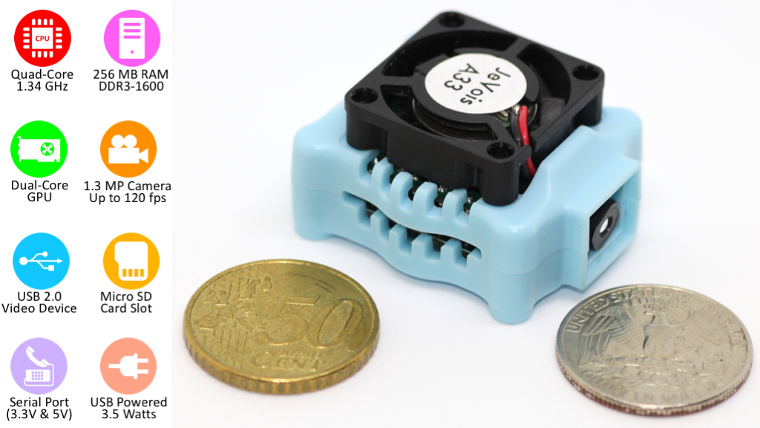
\includegraphics[width=0.5\textwidth]{fig/jevois}
	\caption{JeVois Camera}
	\label{fig:jevois}
\end{figure}

\section{Datasets}
\label{sec:datasets}
An evaluation set has been recorded to serve as a benchmark for the developed methods. The dataset consists of 300 images recorded with the JeVois camera during flight and while remaining on ground. The samples stem from three different rooms with varying light conditions. The rooms are referred to as \textit{Basement}, \textit{Cyberzoo} and \textit{Hallway}. Example images for each room can be seen in \Cref{fig:example_real_set}.
\begin{figure}
	\centering
	\begin{minipage}{0.3\textwidth}
		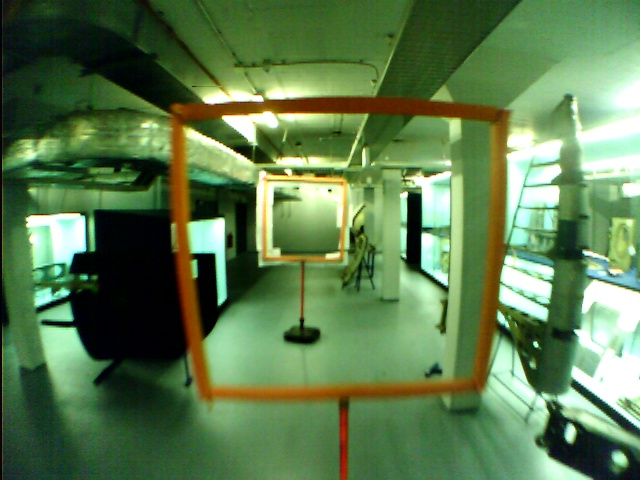
\includegraphics[width=\textwidth]{fig/basement}
	\end{minipage}\hfill
	\begin{minipage}{0.3\textwidth}
	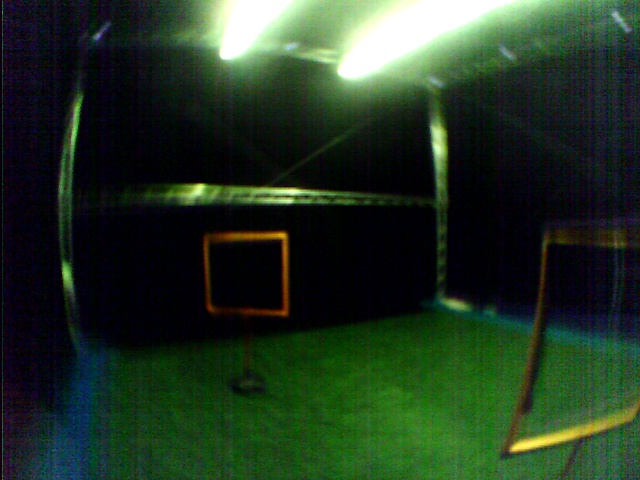
\includegraphics[width=\textwidth]{fig/cyberzoo}
\end{minipage}\hfill
	\begin{minipage}{0.3\textwidth}
	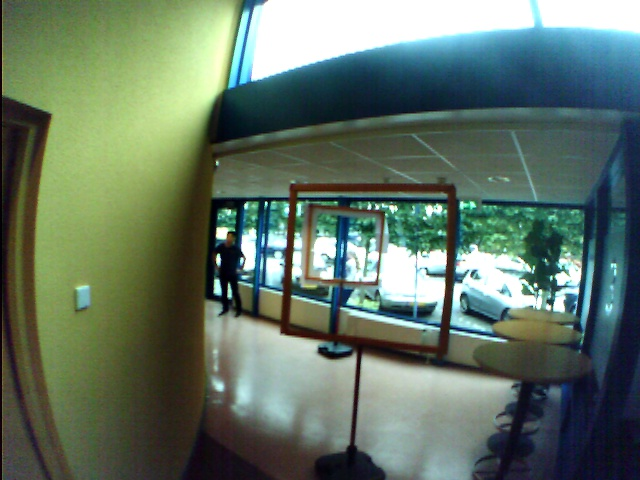
\includegraphics[width=\textwidth]{fig/hallway}
\end{minipage}
\caption{Examples of the three test domains. From left to right: \textit{Basement}, \textit{Cyberzoo} and \textit{Hallway}}
\label{fig:example_real_set}
\end{figure}

All scenes are indoor scenes which are a typical example for a GPS-denied area, where vision based state estimation is required. The scenes contain two gates that are arranged in varying order. Hence up to two objects are visible and can overlap which means the gate farer away can be seen through the closer gate. Each of the rooms has different environmental conditions:
\begin{enumerate}
	\item \textit{Basement} is a bright environment illuminated by artificial light sources. The corridor in which the objects of interest are placed are narrow while also objects and persons are visible on the samples. The dataset contains 163 samples with 312 objects in total.
	\item \textit{Cyberzoo} is taken from a test environment for drone flights. External light sources are covered such that an even illumination and dark background is created. Only in a small subset of images distractors like other objects or persons are visible. In total 88 samples stem from this room while 71 objects are present.
	\item \textit{Hallway} is a bright environment illuminated by a combination of artifical light sources as well as daylight that shines through the windows. The samples are taken with the windows as background. This leads to a very bright background such that the thin structure of the objects are hardly visible. The dataset contains 49 samples with a total of 86 objects.
\end{enumerate}

\section{Evaluation Metrics}

The detection performance is evaluated in terms of precision and recall. These metrics are defined as:

\paragraph{Precision}
$$p = \frac{\text{true positives}}{\text{true positives} + \text{false positives}}$$

\paragraph{Recall}
$$r = \frac{\text{true positives}}{\text{true positives} + \text{false negatives}}$$

Where true positives are objects that are detected, false positives are detections although there is no object and false negatives are objects which have not been detected.

Hence, recall expresses how many of all objects are detected and therefore how complete the result is. Precision measures how many of the predicted objects are actually correct detections.

A correct detection is determined based on its overlap with a ground truth box. This is measured by the relation of \ac{IoU}. In experiments we determine 0.6 as sufficient overlap for a detection. However, to evaluate how accurate in terms of location the detections are, precision and recall are measured for different levels of \ac{IoU}.

The model used within this thesis associates a "confidence" value with each prediction that can trade off precision and recall. This is further explained in \Cref{sec:object_detection}. By accepting more detections with a lower confidence threshold the probability increases that one of the predictions is a true positive. Hence, it increases recall. However, it also increases the probability of false positives and thus lowers precision. In order to evaluate this trade-off precision is plotted over recall at increasing confidence values.

As the learning of \acp{CNN} is stochastic, the mean across several trainings is reported. In order to determine the average precision recall trade-off the precision is interpolated across evenly distributed recall levels between 0 and 1 using:

$$ p_\text{interp}(r) = \max\limits_{r' \geq r} p(r')$$

Subsequently the mean at all recall levels can be calculated. A metric that combines the precision-recall trade-off is \ac{mAP}:


$$ mAP = \int_{r}p_interp(r) dr$$

\todoref{There should be a source for this}

\section{Baseline}

The baseline algorithm \textit{SnakeGate} is a low-level image processing algorithm proposed in \todoref{snakegate}. Its scheme is summarized in and described in the following.

\begin{enumerate}
	\item Filter image by colour threshold
	\item Sample stochastically 
	\item Follow the pixels horizontally as long as they are within the colour threshold otherwise return to 2.
	\item If a bar of sufficient length has been found repeat 3. vertically along one end of the line found in 3.
	\item If a vertical bar is found the square is considered as gate candidate
	\item Create local histogram around the corners of the gate candidate and choose the highest peak as gate corner.
	\item Count the fraction of pixels within the color threshold  in relation to the total number of pixels a long all edges of the gate candidate to determine the \textit{color fitness}.
	\item Gate candidates that exceed a chosen threshold are considered valid detections.
\end{enumerate}
\todo{this can be described more formally}

A property of SnakeGate is that it can and has to be fine tuned given an environment and its corresponding light conditions. This lack of robustness against domain changes are one motivation for this work. On the other hand, in practice the fine tuning allows to adapt the method live for a certain domain, which is not practical for learning based methods.

\subsection{Experiment}

In order to compare the methods investigated in this thesis a baseline is determined. Therefore SnakeGate is evaluated on the datasets described in \Cref{sec:datasets}. In the experiment the color thresholds of the algorithm are fine tuned to the particular environment. The presented results are averages across 5 runs.


\subsection{Results}

The results in terms of precision and recall are summarized in \Cref{fig:snake_results_real}. It can be seen how the detector performs best in the Cyberzoo domain.

\begin{figure}
	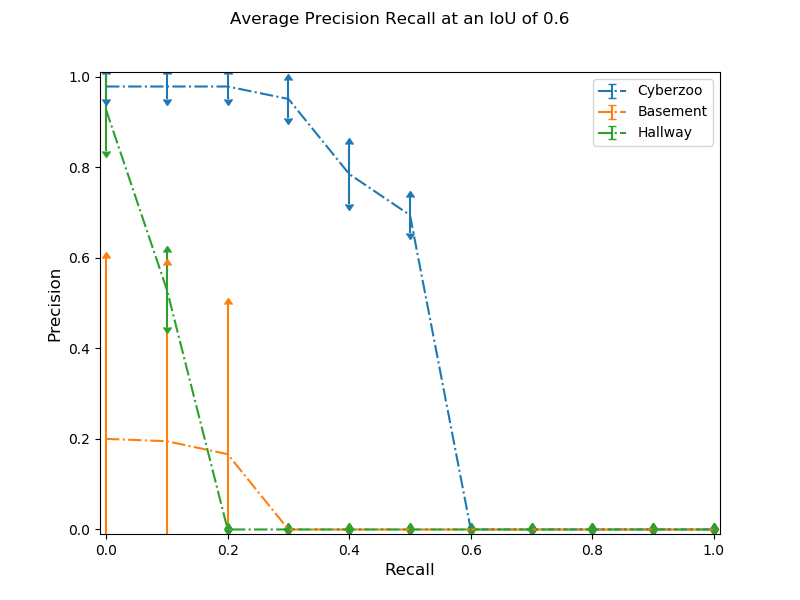
\includegraphics[width=0.8\textwidth]{fig/snake_results_real}
	\caption{Precision-Recall of Snake Gate on the datasets described in \Cref{sec:datasets}}
	\label{fig:snake_results_real}
\end{figure}

